\chapter{Технологическая часть}

В данном разделе рассматривается выбор технологий для реализации поставленной задачи, листинги реализации разработанного программного обеспечения и приведены результаты работы ПО.

\section{Язык программирования}

Для реализации данного проекта выл выбран язык программирования C++ \cite{c++} по нескольким причинам:

\begin{itemize}
	\item[---] наличие для языка C++ необходимых для реализации задачи библиотек;
	\item[---] скорость исполнения кода;
	\item[---] хорошее знание языка C++.
\end{itemize}

\section{ncurses}

Особенностью приложения является то, что работа с терминалом происходит подобно работе с блочным устройством. Это достигается с помощью библиотеки \texttt{ncurses} \cite{ncurses}, предназначенной для управления ввода-вывода на терминал и позволяющей задавать экранные координаты и цвет выводимых символов, реализуется окно терминала на стороне клиента. Библиотека \texttt{ncurses} была выбрана в связи с отсутствием хорошо задокументированных аналогов.

\section{boost}

С помощью набора библиотек \texttt{boost} \cite{boost} реализуется сериализация сообщений которые находятся в пакетах, а так же с запуск команд терминала. Данная библиотека была выбрана из-за большого опыта работы с ней.

\section{Детали реализации}

В листингах \ref{lst:server} - \ref{lst:mutable-state} представлены детали реализации разработанного программного обеспечения.

\subsection{Обработчик сообщений на стороне сервера}

В листинге \ref{lst:server} представлена реализация обработчика сообщений приходящих серверу.\\

\begin{lstlisting}[label=lst:server,caption=Обработчик сообщений (сервер),language=c++]
template <typename Executer>
class MessageProcessor {
	ImmutableState imstate;
	MutableState mstate;
	CursesChProcessor processor;
	Executer executer;
	
	public:
	MessageProcessor() = default;
	bool operator()(const std::vector<char>& data, const int fd, const std::unordered_set<int>& all_fds);
		
	private:
	bool processAddChar(const Message& msg, const int fd, std::unordered_set<int> all_fds);
	bool processGetAll(const int fd);
};

template <typename Executer>
bool MessageProcessor<Executer>::operator()(const std::vector<char>& data, const int fd, const std::unordered_set<int>& all_fds)
{
	const std::string s(data.begin(), data.end());
	auto message = Message(s);
	switch (message.type) {
		case Message::Type::addChar:
			return processAddChar(message, fd, all_fds);
		case Message::Type::getAll:
			return processGetAll(fd);
		default:
			return false;
	}
	return false;
}

template <typename Executer>
bool MessageProcessor<Executer>::processAddChar(const Message& msg, const int fd, std::unordered_set<int> all_fds)
{
	auto m = AddCharMessage(msg.data);
	mstate.setCurpos(m.pos);
	auto res = processor.process(imstate, mstate, m.data);
	
	std::string packet;
	if (res == CursesChProcessor::ActionType::Exec) {
		auto command = mstate.getData();
		auto res = executer.execute(command);
		
		res.insert(res.begin(), "> " + command);
		for (auto& s : res)
		imstate.insertLine(s);
		
		auto diffMessage = DiffMessage(res);
		auto message = diffMessage.buildMessage();
		packet = message.buildPacket();
	} else {
		packet = msg.buildPacket();
	}
	
	if (res != CursesChProcessor::ActionType::BadKey)
		broadcastPacket(packet, all_fds);
	
	return true;
}

template <typename Executer>
bool MessageProcessor<Executer>::processGetAll(const int fd)
{
	auto message = GetAllMessage(imstate, mstate);
	auto msg = message.buildMessage();
	auto packet = msg.buildPacket();
	if (send(fd, packet.data(), packet.size(), 0) == -1) {
		std::cout << "Can't send data to client\n";
		return false;
	}
	return true;
}
\end{lstlisting}

\subsection{Обработчик сообщений на стороне клиента}

В листинге \ref{lst:client} представлена реализация обработчика сообщений на стороне клиента.\\

\begin{lstlisting}[label=lst:client,caption=Обработчик сообщений (клиент),language=c++]
class MessageProcessor {
	public:
	void operator()(ImmutableState& imstate, MutableState& mstate, Message msg);
	
	private:
	void movePos(MutableState& msate, const std::size_t old_pos, const std::size_t pos, const int data);
};

void MessageProcessor::operator()(ImmutableState& imstate, MutableState& mstate, Message msg)
{
	if (msg.type == Message::Type::addChar) {
		const auto message = AddCharMessage(msg.data);
		const auto old_pos = mstate.getCurpos();
		
		mstate.setCurpos(message.pos);
		if (is_backspace(message.data))
			mstate.removeChar();
		else
			mstate.addChar(static_cast<char>(message.data));
			movePos(mstate, old_pos, message.pos, message.data);
		
	} else if (msg.type == Message::Type::diff) {
		auto message = DiffMessage(msg.data);
		mstate.getData();
		imstate.insertLines(std::move(message.diff));
	}
}

void MessageProcessor::movePos(MutableState& mstate, const std::size_t old_pos, const std::size_t pos, const int data)
{
	std::size_t new_pos;
	if (data == KEY_BACKSPACE || data == 127 || data == KEY_DC)
		new_pos = (old_pos >= pos && old_pos > 0) ? old_pos - 1 : old_pos;
	else
		new_pos = (old_pos < pos) ? old_pos : old_pos + 1;
	mstate.setCurpos(new_pos);
}
\end{lstlisting}

\subsection{Базовые структуры сообщения}

Сообщение, передаваемое в теле пакета, описывается некоторой структурой. Эти структуры и их методы описаны в листинге \ref{lst:message-struct}.\\ 

\begin{lstlisting}[label=lst:message-struct,caption=Базовые структуры\, описывающие сообщение,language=c++]
struct Message {
	enum class Type : std::uint8_t {
		addChar,
		getAll,
		diff,
	};
	
	Type type;
	std::string data;
	
	Message() = default;
	Message(const std::string& s);
	Message(Message::Type type, const std::string&& s);
	std::string buildPacket() const;
	template <typename Archive>
	void serialize(Archive& ar, const unsigned int version);
};

struct AddCharMessage {
	std::size_t pos;
	int data;
	
	template <typename Archive>
	void serialize(Archive& ar, const unsigned int version);
	AddCharMessage(const std::string& s);
	AddCharMessage(const int data, const std::size_t pos);
	Message buildMessage() const;
};

struct DiffMessage {
	std::vector<std::string> diff;
	
	template <typename Archive>
	void serialize(Archive& ar, const unsigned int version);
	DiffMessage(const std::string& s);
	DiffMessage(const std::vector<std::string>& diff);
	Message buildMessage() const;
};

struct GetAllMessage {
	ImmutableState imstate;
	MutableState mstate;
	
	template <typename Archive>
	void serialize(Archive& ar, const unsigned int version);
	GetAllMessage(const std::string& s);
	GetAllMessage(const ImmutableState& imstate, const MutableState& mstate);
	Message buildMessage() const;
};

template <typename Archive>
void Message::serialize(Archive& ar, const unsigned int version)
{
	ar& type;
	ar& data;
}

Message::Message(const std::string& s)
{
	std::istringstream ins(s);
	boost::archive::binary_iarchive in(ins);
	in >> *this;
}

Message::Message(Message::Type type, const std::string&& s)
: type(type)
, data(std::move(s))
{
}

std::string Message::buildPacket() const
{
	std::ostringstream outs;
	
	boost::archive::binary_oarchive out(outs);
	out << *this;
	auto res = outs.str();
	
	char buf[4];
	size_to_char(res.size(), buf);
	std::string prefix = { buf, 4 };
	return prefix + res;
}

template <typename Archive>
void AddCharMessage::serialize(Archive& ar, const unsigned int version)
{
	ar& pos;
	ar& data;
}

AddCharMessage::AddCharMessage(const std::string& s)
{
	std::istringstream ins(s);
	boost::archive::binary_iarchive in(ins);
	in >> *this;
}

AddCharMessage::AddCharMessage(const int data, const std::size_t pos)
: pos(pos)
, data(data)
{
}

Message AddCharMessage::buildMessage() const
{
	std::ostringstream outs;
	boost::archive::binary_oarchive out(outs);
	out << *this;
	return Message { Message::Type::addChar, outs.str() };
}

template <typename Archive>
void DiffMessage::serialize(Archive& ar, const unsigned int version)
{
	ar& diff;
}

DiffMessage::DiffMessage(const std::vector<std::string>& diff)
: diff(diff)
{
}

DiffMessage::DiffMessage(const std::string& s)
{
	std::istringstream ins(s);
	boost::archive::binary_iarchive in(ins);
	in >> *this;
}

Message DiffMessage::buildMessage() const
{
	std::ostringstream outs;
	boost::archive::binary_oarchive out(outs);
	out << *this;
	return Message { Message::Type::diff, outs.str() };
}

template <typename Archive>
void GetAllMessage::serialize(Archive& ar, const unsigned int version)
{
	ar& imstate;
	ar& mstate;
}

GetAllMessage::GetAllMessage(const std::string& s)
{
	std::istringstream ins(s);
	boost::archive::binary_iarchive in(ins);
	in >> *this;
}

Message GetAllMessage::buildMessage() const
{
	std::ostringstream outs;
	boost::archive::binary_oarchive out(outs);
	out << *this;
	return Message { Message::Type::getAll, outs.str() };
}

GetAllMessage::GetAllMessage(const ImmutableState& imstate, const MutableState& mstate)
: imstate(imstate)
, mstate(mstate)
{
}
\end{lstlisting}

\subsection{Состояния системы}

Система содержит в себе два состояния: изменяемое и неизменяемом:

\begin{itemize}
	\item[---] изменяемое состояние -- строка, которую могут редактировать текущие клиенты;
	\item[---] неизменяемое состояние -- содержит информацию о запущенных командах и их выводе.
\end{itemize} 

Неизменяемое состояние -- состояние когда исполняется какая-либо команда, введенная пользователем, при этом все введенные пользователем символы записываются в специальный буффер и обрабатываются после исполнения команды.

В листингах \ref{lst:immutable-state} и \ref{lst:mutable-state} представлена реализация неизменяемого и изменяемого состояния.\\

\begin{lstlisting}[label=lst:immutable-state,caption=Класс\, описывающий неизменяемое состояние системы,language=c++]
class ImmutableState {
	std::size_t startline = 0;
	std::vector<std::string> data;
	
	public:
	std::size_t printLines(
	const std::size_t max_lines = std::numeric_limits<std::size_t>::max(),
	const std::size_t offset = 0) const;
	void insertLine(const std::string& s);
	void insertLines(std::vector<std::string>&& vs);
	void moveUp(const std::size_t diff = 1);
	void moveDown(const std::size_t diff = 1);
	std::size_t linesToShow();
	void setLinesToShow(const std::size_t lines);
	
	private:
	friend class boost::serialization::access;
	template <typename Archive>
	void serialize(Archive& ar, const unsigned int version)
	{
		ar& data;
	}
};

std::size_t ImmutableState::printLines(
const std::size_t max_lines,
const std::size_t offset) const
{
	auto limit = std::min(max_lines, data.size() - startline);
	for (std::size_t i = 0; i < limit; i++) {
		move(i + offset, 0);
		clrtoeol();
		printw("%s", data[i + startline].c_str());
	}
	return limit;
}

void ImmutableState::insertLine(const std::string& s)
{
	data.push_back(s);
}

void ImmutableState::insertLines(std::vector<std::string>&& vs)
{
	for (std::size_t i = 0; i < vs.size(); i++)
	data.push_back(std::move(vs[i]));
}

void ImmutableState::moveUp(const std::size_t diff)
{
	startline = diff > startline ? 0 : startline - diff;
}

void ImmutableState::moveDown(const std::size_t diff)
{
	startline = std::min(data.size(), startline + diff);
}

std::size_t ImmutableState::linesToShow()
{
	return data.size() - startline;
}

void ImmutableState::setLinesToShow(const std::size_t lines)
{
	startline = data.size() > lines ? data.size() - lines : 0;
}
\end{lstlisting}

\begin{lstlisting}[label=lst:mutable-state,caption=Класс\, описывающий изменяемое состояние системы,language=c++]
#define PROMPT "> "
#define PROMPT_SIZE 2

class MutableState {
	std::string data;
	std::size_t curpos = 0;
	
	public:
	std::size_t getCurpos() const;
	void setCurpos(const std::size_t new_curpos);
	
	void printLine(const std::size_t yoffset = 0) const;
	void addChar(const char c);
	void removeChar();
	void moveLeft(const std::size_t diff = 1);
	void moveRight(const std::size_t diff = 1);
	const std::string& getText() const;
	void clearData();
	std::string getData();
	
	private:
	friend class boost::serialization::access;
	template <typename Archive>
	void serialize(Archive& ar, const unsigned int version)
	{
		ar& data;
	}
};

std::size_t MutableState::getCurpos() const { return curpos; }

void MutableState::setCurpos(const std::size_t new_curpos)
{
	curpos = std::min(new_curpos, data.size());
}

void MutableState::printLine(const std::size_t yoffset) const
{
	move(yoffset, 0);
	clrtoeol();
	printw(PROMPT "%s", data.c_str());
	move(yoffset, PROMPT_SIZE + curpos);
}

void MutableState::addChar(const char c)
{
	data.insert(data.begin() + curpos++, c);
}

void MutableState::removeChar()
{
	if (curpos > 0)
	data.erase(--curpos, 1);
}

void MutableState::moveLeft(const std::size_t diff)
{
	curpos = diff > curpos ? 0 : curpos - diff;
}

void MutableState::moveRight(const std::size_t diff)
{
	curpos = std::min(data.size(), curpos + diff);
}

const std::string& MutableState::getText() const { return data; }

void MutableState::clearData()
{
	curpos = 0;
	data.clear();
}

std::string MutableState::getData()
{
	curpos = 0;
	auto old_data = std::move(data);
	data.clear();
	return old_data;
}
\end{lstlisting}

\section{Примеры работы разработанного ПО}

В листингах \ref{fig:example_01} и \ref{fig:example_02} представлены результаты работы разработанного программного обеспечения.

\begin{center}
	\begin{figure}[h]
		\begin{center}
			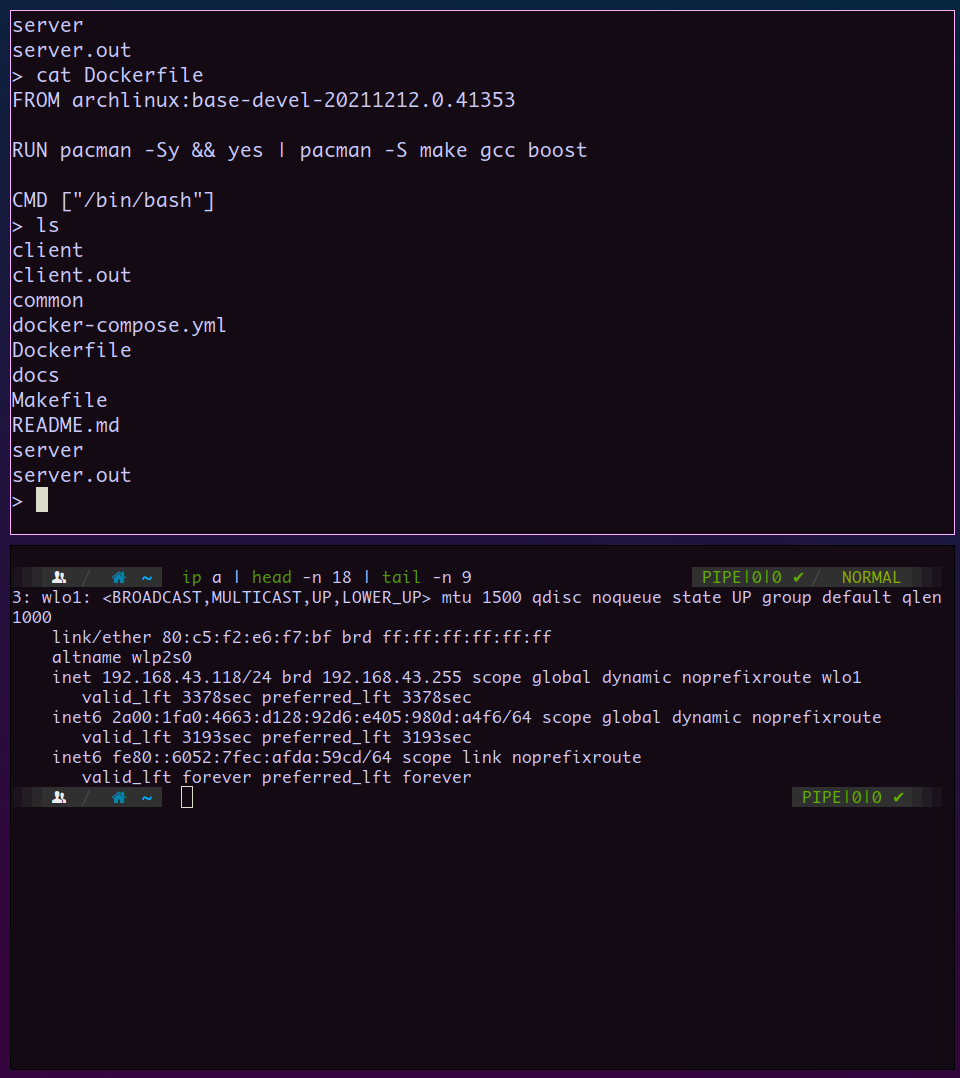
\includegraphics[scale=0.5]{img/example_01.png}
		\end{center}
		\caption{\label{fig:example_01} Вывод сервера и его IP адрес}
	\end{figure}
\end{center}

\begin{center}
	\begin{figure}[h]
		\begin{center}
			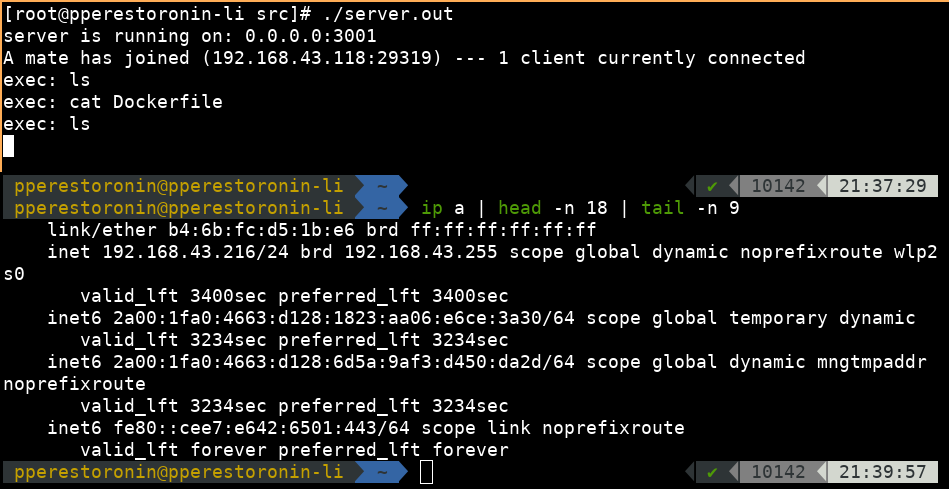
\includegraphics[scale=0.5]{img/example_02.png}
		\end{center}
		\caption{\label{fig:example_02} Вывод клиента и его IP адрес}
	\end{figure}
\end{center}


\section*{Вывод}

В данном разделе был обоснован выбор технологий для решения поставленной задачи, рассмотрены листинги реализованного программного обеспечения и приведены результаты работы ПО.